\section{Classification}
Sentence classification is a natural language processing task that involves assigning a predefined category or label to a given sentence. One way to approach sentence classification is to use word embeddings, which are numerical representations of words that capture their meaning and context within a sentence. Word embeddings can be generated using various techniques, such as training a neural network on a large dataset of text or using a pre-trained language model. \\
Once the word embeddings have been generated, you can input them into a classifier along with other features of the sentence, such as its grammatical structure, to make predictions about the sentence's category or label. The classifier uses the word embeddings as input to make predictions about the sentence's category or label. \\
We used two different pre-trained language model: BERT and fastText. We chose BERT because it is a widely used and well-studied model, and our objective was not to find the absolute best classifier, but only to show that the dataset could be used as training data. \\
Instead, we chose fastText to have an option which was CPU-friendly, and that could be trained in a matter of a few minutes. \\
The training data used were the texts of the 16000 tickets that compose the HR ticket dataset, whereas the test data were the survey tickets. The labels were the combination of ticket category and ticket subcategory of each ticket ( Ex. "Life event\_Health issues").


\subsection{FastText Classifier}
FastText is a library developed by Facebook AI Research that provides a set of training algorithms for supervised learning of word embeddings from raw text and also can be used to build and train supervised text classification models. \\
FastText creates word embeddings using a combination of character n-grams and word n-grams. To do this, fastText first breaks each word in the training text into its constituent character n-grams. For example, the word "cat" might be broken into the character n-grams "c", "ca", "cat", "a", "at", and "t". These character n-grams are then used to generate vectors. The word embeddings are calculated as the sum of their n-gram vectors. \\
To learn the embeddings of these n-grams, fastText uses a skip-gram model, which is a type of model that maximizes the probability of observing a word given its context, or in other words its surrounding words. By using this approach, fastText is able to learn high-quality word embeddings that capture the syntactic and semantic information of words. \\
The fastText classification uses the fastText embeddings as input to the model, and in particular:
\begin{algorithm}
    \caption*{fastText Classification}
    \begin{algorithmic}[1]
      \State Words representation are averaged into a text representation
      \State The text representation is fed to a linear classifier
      \State The output of the linear classifier is given as input to a softmax function to compute the probability distribution over a set of predefined classes
    \end{algorithmic}
\end{algorithm}


\subsection{BERT classifier}
BERT (Bidirectional Encoder Representation from Transformers) is a model developed by Google AI based on the transformers architecture. BERT was trained on a large corpus on two different tasks: Masked Language Modeling and Next Sentence Prediction. \\
Through the use of MLM, in the training phase, 15\% of the tokens in a sentence are obscured and BERT can then be utilized to utilize the surrounding words in both directions to predict the masked tokens, facilitating bidirectional learning from the text. \\
On the other hand, NSP helps the model understand the relationships between sentences. Specifically, in the training phase, 50\% of the examples are actually successive sentences, while in the other 50\% of the cases this condition is not respected. \\
BERT is quite straightforward to fine-tune, we just need to plug in the necessary layers at the top of the BERT architecture and fine-tune for a sufficient number of epochs the model end-to-end. \\
The first token of a BERT embedding is the [CLS] token, which is a special token that acts as an aggregate representation of the sentence. The final embedding of the [CLS] token is used as input for the classification task. The most simple method, which is also the method used by the BERTForSequenceClassification class by HuggingFace, is to take the embedding of the [CLS] token at the last hidden layer and fed it to a single layer of a feed-forward network. The layer of the feed-forward network will have n input, where n is the dimension of the embedding of a token, and m output, where m is the desired number of outputs. \\
The final model is shown in \autoref{fig:bert_class}
\begin{figure}[h] 
  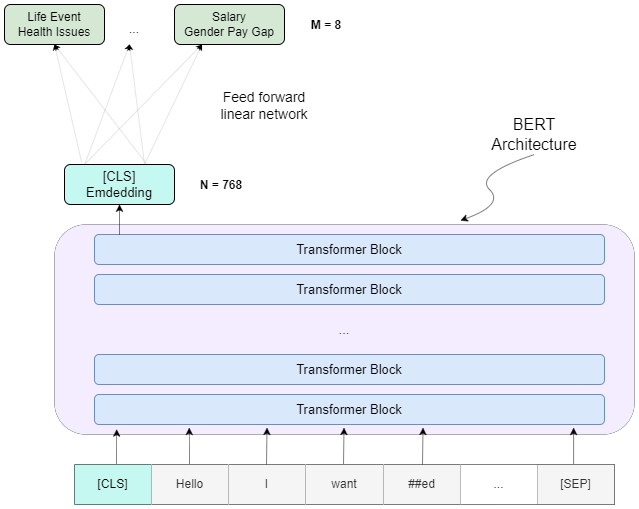
\includegraphics[width=\textwidth]{images/bert_class.drawio.png}
  \caption{Schema of BERT classification}
  \label{fig:bert_class}
\end{figure}

\subsection{Results}
In this section we show the results of the classification experiments. We want to reiterate that the point of the experiments was not to get the best possible results, therefore the models were not trained for a large amount of epochs and we did not try an excessive number of possible hyperparameters.
The hyperparameters tried are shown in \autoref{table:hyp_fasttext} and \autoref{table:hyp_bert}. If an hyperparameter is not shown in the table it means we have used its default value. \\
The technique used for finding the optimal hyperparameters is Grid Search, which means we have trained and tested the models for each combination of all the chosen values of the hyperparameters to determine the hyperparameters' set which achieves the best results.

\begin{table}[h]
  \begin{tabular}{|l|l|}
  \hline
  Size of context window (ws)                   & 5      \\ \hline
  epochs                                        & 20     \\ \hline
  minimal number of word occurencies (minCount) & 1      \\ \hline
  max length of word ngram (wordNgrams)         & 3      \\ \hline
  learning rate (lr)                            & 0.5    \\ \hline
  learning update rate (lrUpdateRate)           & 100    \\ \hline
  sampling threshold (t)                        & 0.0001 \\ \hline
  \end{tabular}
  \caption{Hyperparameters fastText}\label{table:hyp_fasttext}
\end{table}

\begin{table}[h]
  \begin{tabular}{|l|l|}
  \hline
  epochs           & {[}3, 5{]}                              \\ \hline
  learning rate    & {[}1e-05, 5e-04, 1e-04, 5e-05, 5e-06{]} \\ \hline
  weight decay     & {[}0.001, 0.01, 0.05{]}                 \\ \hline
  train batch size & {[}8, 16{]}                             \\ \hline
  warmup steps     & 500                                     \\ \hline
  \end{tabular}
  \caption{Hyperparameters BERT}\label{table:hyp_bert}
  \end{table}

%TODO: add results
As we expected, fastText performs worse than BERT, achieving an $f_1$ score of only 0.41. \\
On the other hand, the BERT classifier with hyperparameters\begin{itemize}
  \item epochs: 5
  \item learning rate: 5e-05
  \item weight decay: 0.001
  \item train batch size: 8
  \item warmup steps: 500
\end{itemize}
achieved an $f_1$ score of 0.78. We show also the confusion matrix( \autoref{fig:conf_matrix_bert_class} ) to highlight how the majority of errors comes from two sub-categories that belong to the same category, in particular "Gender wage gap"-"Salary raise" and "Personal issues"-"Health issues". In some way, this validates our initial decision on the taxonomy of the tickets.
\begin{figure}[h] 
  \centering
  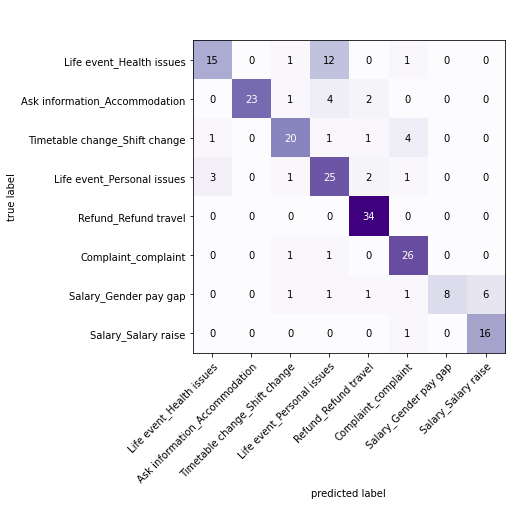
\includegraphics[width=0.8\textwidth]{images/conf_matrix_bert_class.png}
  \caption{Confusion matrix of Ticket classification with BERT}
  \label{fig:conf_matrix_bert_class}
\end{figure}    
